\documentclass[10pt]{IEEEtran}

\usepackage[utf8x]{inputenc}
\usepackage[L7x]{fontenc}
\usepackage[lithuanian]{babel}
\usepackage{listings}
\usepackage{graphicx}
\usepackage{epstopdf}

\lstset{
	basicstyle=\footnotesize,
	language=Java,
	morekeywords={String,each,in,Iterator}
}

\author{Maksim Norkin\\ \texttt{maksim.norkin@ieee.org}}
\title{Projektavimo šablonai \\ \footnote{Design Patterns}}

\begin{document}

	\maketitle

	\section{Įžanga}

		Programų inžinerijoje, projektavimo šablonas yra bendras, daug kartų naudojamas sprendimas nuolat kylančiai problemai išspręsti. Projektavimo šablonas nėra galutinis programinės įrangos sprendimas. Tai yra šablonas arba aprašymas kaip galima išspręsti kažkokią problemą skirtingose situacijose. Šablonus galima pervadinti į sprendimų rinkinius, kurie yra išgryninti programuotojų bendruomenės ir sąlygoja geriausią sprendimą. Objektiškai orientuoti projektavimo šablonai dažniausiai nurodo susiejimus ir sąveikas tarp klasių arba objektų, nesileidžiant į galutinių objektų ar klasių aprašymo. Daugelis šablonų įgyvendina objektiškai orientuotą arba paveldimą būseną, todėl jie gali būti neįmanomi pritaikyti funkciniame programavime. 

		Projektavimo šablonai priklauso modulių ir sujungimų srityje. Aukštesniam lygmenyje yra naudojami architektūriniai šablonai, kurie dažniausiai nusako bendrą šabloną, kurio privalo laikytis visa likusi sistema.

		Egzistuoja labai daug projektavimo šablonų, pavyzdžiui:

		\begin{itemize}
			\item Algoritminės strategijos šablonai, kurie nusako galimus sprendimus, kurie yra susiję su aukšto lygio strategijomis -- kaip išnaudoti programos charakteristikas skaičiavimo mašinoje.
			\item Skaičiuojamieji projektavimo šablonai, kurie nusako svarbiausius skaičiavimo proceso vietas.
			\item Paleidimo šablonas, nusako programos paleidimo palaikymą, įtraukiant strategijas, kurios nusako kaip paleisti programinės sistemos srautus, taip remiant užduočių sinchronizavimą.
			\item Įgyvendinimo strategijos šablonai, nusako kaip galima pateikti programinį kodą programos organizavimui ir bendrus duomenų tipus, konkrečiai lygiagrečiam programavimui.
			\item Struktūriniai projektavimo šablonai, nusako kaip galima įvykdyti aukšto lygio struktūras programos kūrimo metu.
		\end{itemize}

	\section{Istorija}

		Šablonai atsirado kaip architektūrinė idėją, kurią pristatė Christopher Alexander. 1987 metais, Kent Beck ir Ward Cunningham pradėjo idėjos eksportavimą į kitas šakas, tarp kurių ir programavimas. Savo darbo rezultatus Jie paskelbė OOPSLA konferencijoje tais pačiais metais. Vėlesniais metais, jų darbas buvo tęsiamas toliau.

		Projektavimo šablonai gavo labai didelį populiarumą kompiuterių moksle, kai 1994 buvo išleista knyga ``Design Patterns: Elements of Reusable Object-Oriented Software'', kurių autoriai yra ``Gang of Four'' (Gamma et al.), kurie dažniausiai yra trumpinami iki ``GOF''. Tais pačiais metais, buvo surengta pirmoji \textit{Pattern Languages of Programming} konferencija. Sekančiais metais, buvo įsteigta \textit{Portland Pattern Repository}, kurios paskirtis buvo projektavimo šablonų dokumentavimas. 

		Turint omenyje, kad projektavimo šablonai buvo taikomi praktikoje labai ilgą laiką, formalus jų aprašymas yra nyksta jau keletas metų.

		Tik 2009, Tomas Erl kartu su 30 inžinierių vieningomis jėgomis išleido knygą ``SOA Design Patterns'', kurios tikslas buvo nustatyti \textit{de facto} projektavimo šablonų apibūdinimus SOA ir paslaugų tipo sprendimams.

	\section{Praktika}

		Projektavimo šablonai gali labai paspartinti darbo procesą, pateikdami išbandytus, įrodytus projektavimo pavyzdžius. Efektyvus programinio paketo šablonas reikalauja turėti omenyje problemas, kurios gali nepasirodyti iki tada, kai žymi darbo dalis jau bus atlikta. Projektavimo šablonų pakartotinis taikymas leidžia išvengti subtilių problemų, kurios gali peraugti į dideles problemas. Taip pat yra pagerinamas kodo skaitymas programuotojams ir architektams, kurie jau turi projektavimo šablonų žinių.

		Projektavimo šablonai dažniausiai įveda papildomus netiesioginius lygius, kuomet reikia lankstumo. Kai kuriais atvejais tai gali sukelti atlikimo spartos sumažėjimą.

		Remiantis projektavimo šablono sąvoka, projektavimo šablonai turi būti iš naujo realizuojami kiekvienoje naujoje situacijoje. Kai kurie autoriai nusprendė, kad toks darbo pobūdis yra žingsnis atgal nuo pakartotinio programinio kodo panaudojimo, kaip yra daroma modulinio programavimo atveju, projektavimo šablonai buvo perdaryti moduliniu pagrindu. Meyer ir Arnout sugebėjo panaudoti arba pilną, arba dalinį komponentų panaudojimą, tais projektavimo atvejais, kuriais jie taikė projektavimo šablonus.

	\section{Klasifikavimas}

		Pradžioje projektavimo šablonai buvo sugrupuoti į kategorijas: kūrimo šablonai, struktūriniai šablonai ir elgesio šablonai. 

		\subsection{Kūrimo šablonai}

			\begin{itemize}
				\item \textit{Abstract factory} -- sukuria sąsaja panašios šeimos ar susijusių objektų, jų priklausomybių kūrimui, nenusakant tiksliai visų reikalavimų.
				\item \textit{Builder} -- sudėtingo konstruktoriaus atskyrimas nuo jo pateikimo, leidžiant skirtingus objektus kurti su tuo pačiu konstruktoriumi.
				\item \textit{Factory method} -- objektų kūrimo sąsajos įgyvendinimas, kur dukterinė klasė nusprendžia kokia klasė yra paveldima.
				\item \textit{Lazy initialization} -- taktinis objekto kūrimo, sudėtingo skaičiavimo ar kito sudėtingo proceso paleidimo užlaikymas iki tada, kai jo prireikia.
				\item \textit{Multiton} -- klasės baigtinių egzempliorių užtikrinimas ir globalus jų priėjimas.
				\item \textit{Object pool} -- šablonas nusako, kaip elgtis norint išvengti sudėtingų išteklių priskyrimų ir paleidimo, kuomet jie nėra reikalingi.
				\item \textit{Prototype} -- nusakoma kokio tipo objektus sukurti, naudojantis prototipo egzemplioriumi. Taip pat galima klonuoti objektus, kopijuojant esamą prototipo egzempliorių.
				\item \textit{Resource acquisition} -- šablonas užtikrina resursų atlaisvinimu, kuomet jie nėra reikalingi, surišdamas juos su objektų gyvavimo trukme.
				\item \textit{Singleton} -- vieno objekto egzemplioriaus užtikrinimas. Taip pat pridedamas globalus priėjimas prie duoto objekto.
			\end{itemize}

		\subsection{Struktūriniai šablonai}

			\begin{itemize}
				\item \textit{Adapter} -- sąsajos konvertavimas iš vienos, kurios klientas nesupranta, į tą, kurią jis supranta. Adapteris leidžia objektams bendrauti kartu, kas būtų neįmanoma dėl nesutampančių sąsajų.
				\item \textit{Bridge} -- abstrakcijos priklausomybių (angl. \textit{decoupling}) atskyrimas nuo jos realizacijos, taip sudarant lankstumo sąlygas.
				\item \textit{Composite} -- objektų sudarymas į medžio šakas, siekiant pateikti atskiro modulio ar visos sistemos hierarchiją. \textit{Composite} leidžia klientams vienodai elgtis tiek su vienu objektu, tiek su objekto medžiu.
				\item \textit{Decorator} -- dinaminis papildomos atsakomybės priskyrimas prie objekto, paliekant tą pačią sąsają. \textit{Decorator} yra labai gera alternatyva klasės paveldėjimui.
				\item \textit{Facade} -- subendrintos sąsajos pateikimas sąsajų grupės posistemei. \textit{Facade} apibrėžia aukšto lygio sąsają, kuri leidžia lengvai naudotis posisteme.
				\item \textit{Flyweight} -- efektyvus panašių objektų dalinimas tarp sistemos.
				\item \textit{Front Controller} -- centralizuoto įrašo pateikimas, apdorojant užklausas.
				\item \textit{Module} -- grupė susijusių elementų: klasės, singleton'ai, metodai, naudojami globaliai, iš vieno bendro taško.
				\item \textit{Proxy} -- pakaitalo ar rezervato patekimas objekto kontrolei.
			\end{itemize}

		\subsection{Elgesio šablonai}

			\begin{itemize}
				\item \textit{Blackboard} -- daugelio rašytojų/skaitytojų suteikimas, subendrinant stebėtoją. Duomenų perdavimas atliekamas visos sistemos atžvilgiu.
				\item \textit{Chain of responsibility} -- Vengimas siuntimą priskirti kažkokiam vienam objektui. Keliama galimybė keliems objektams apdoroti ateinančią informaciją.
				\item \textit{Command} -- užklausos yra pateikiamos kaip uždari objektai, kas leidžia klientams pateikti skirtingas užklausas, eiles ar žurnalą.
				\item \textit{Interpreter} -- turint kalbą, apibūdinti jos žodyną kartu su interpretatoriumi, kuris naudoja žodyną ir supranta kalbos sakinius.
				\item \textit{Iterator} -- pateikti sprendimą, kaip galima pateikti visus esamo objekto elementus, nesigilinant į objekto vidinę struktūrą.
				\item \textit{Mediator} -- nurodyti objektą, kuris reguliuoja kaip objektų grupę tarpusavyje sąveikauja. \textit{Mediator} skatina laisvą jungimą, taip išvengiant tiesioginį vieno objekto priklausomybę nuo kito objekto, kurie priklauso \textit{mediator} objektui. 
				\item \textit{Memento} -- leidimas objekto būsenos atstatymui uždelstam laike, nepažeidžiant objekto priklausomybių.
				\item \textit{Null object} -- null tipo vengimas, priskiriant reikšmę kūrimo metu.
				\item \textit{Observer} -- apibūdinti vienas-daugelis sąryšį, kur vieno objekto atnaujinimas skatina jam priklausančių objektų automatinį atnaujinimą.
				\item \textit{Servant} -- objektų grupės bendro funkcionalumo aprašymas.
				\item \textit{Specification} -- loginiais ryšiais jungiama verslo logika.
				\item \textit{State} -- leidimas objektui keisti jo elgesį, pasikeitus jo vidiniai būsenai. Objektas gali pakeisti savo klasę.
				\item \textit{Strategy} -- algoritmo šeimos apibūdinimas, vieno kito paveldėjimas ir priklausomybė. \textit{Strategy} leidžia keisti algoritmus, priklausomai nuo kliento kreipinio.
				\item \textit{Template method} -- operacijos skaldymas į dukterines klases, pradžioje aprašant tik algoritmo griaučius. Metodas leidžia dukterinėms klasėms iš naujo deklaruoti tam tikras operacijas iš naujo, nekeičiant bendro algoritmo logikos.
				\item \textit{Visitor} -- pateikia operacijas, kurios yra įvykdomos su objekto elementais. \textit{Visitor} leidžia pateikti naują operaciją, nepakeičiant jo operuojamų elementų klases. 
			\end{itemize}

		\subsection{Lygiagretumo šablonai}

			\begin{itemize}
				\item \textit{Active Object} -- atskiria metodo iškvietimą nuo metodo kreipinio, kuris egzistuoja kontroliuojamoje šakoje. Tikslas yra pateikti lygiagretumą, naudojant asinchroninius kreipinių iškvietimą ir kontroliuojamą užklausų apdorojimą.
				\item \textit{Balking} -- objekto operacija kviečiama tik tuomet, kai objektas yra tam tikroje būsenoje.
				\item \textit{Binding properties} -- priverstinis savybių sinchronizavimas tarp stebėtojų, juos sujungiant.
				\item \textit{Double-checked locking} -- lengvinamas užrakto gavimas, pirmiausia bandant uždarymo kriterijų nesaugioje būsenoje. Jeigu bandymas sėkmingas -- resursas užrakinamas. Toks šablonas gali būti nesaugus, todėl jį galima traktuoti kaip priešpriešinis šablonas.
				\item \textit{Event-based asynchronous} -- problemų adresavimas ne sinchroniniam režime. Nutinka lygiagrečiose programose.
				\item \textit{Guarded suspension} -- valgo veiksmus, kuriems riekia rakto ir tam tikros sąlygos, norint jas įvykdyti.
				\item \textit{Lock} -- vienos gijos rakto uždėjimas ant tam tikro resurso. Tokiu atveju kitos gijos negali prieiti prie resurso, kol nebus paleistas raktas.
				\item \textit{Messaging} -- leidžia informacijos perdavimą tarp sistemos modulių ir komponenčių.
				\item \textit{Monitor object} -- objekto metodų kontroliuojamas paleidimas. Taip išvengiama kelių objekto metodų kreipinių lygiagrečioje sistemoje. 
				\item \textit{Reactor} -- Rektoriaus objektas suteikia ne sinchroninį priėjimą prie duomenų, kai juos reikia pateikti sinchroniškai.
				\item \textit{Read-write lock} -- suteikti galimybę skaityti iš objekto laisvai, tačiau rašymo operacijai reikalingos ypatingos teisės.
				\item \textit{Scheduler} -- labai griežtas vienos gijos metodų paleidimas, kelių gijų skaitymo atveju.
				\item \textit{Thread pool} -- sukuriamas tam tikras gijų skaičius, organizuotas į eilę, operacijai atlikti. Specialus \textit{Object pool} atvejis.
				\item \textit{Thread-specific storage} -- statinės ar globalinis priėjimas prie lokalių gijos duomenų.
			\end{itemize}

	\section{Kūrimo šablonai}

		\subsection{Kūrimo šablonas}

			Programų inžinerijoje, kūrimo šablonai yra specialūs projektavimo šablonai, kurių paskirtis yra kontroliuoti objektų sukūrimą, priklausomai nuo tam tikrų aplinkybių. Paprasčiausias objekto sukūrimas gali privesti prie projektavimo problemų ar pridėti labai daug nereikalingo kompleksiškumo. Kūrimo šablonai sprendžia šitą problemą, pateikiant kontrolės mechanizmus objekto kūrimui.

			Kūrimo šablonai susideda iš dviejų pagrindinių idėjų:
			\begin{itemize}
				\item Sistemos naudojamų klasių sąrašo pateikimas
				\item Slėpti sistemos naudojamų modelių kūrimo ir jų sujungimo logiką 
			\end{itemize}

			Kūrimo šablonai gali būti suskirstyti toliau į objekto kūrimo šablonus ir klasės kūrimo šablonus. Objekto kūrimo šablonai daugiau orientuoti objektui priklausančių objektų kūrimą, o klasės kūrimo šablonai rūpinasi objekto kūrimui dukterinėse klasėse.

			Penki labiausiai žinomi projektavimo šablonai yra:

			\begin{itemize}
				\item \textit{Abstract factory}, kuris leidžia kurti objektus, nesirūpinant objekto priklausomybėmis.
				\item \textit{Builder} šablonas, kuris atskiria sudėtingo projekto konstrukciją nuo jo atvaizdavimo.
				\item \textit{Factory method}, kuris leidžia nesirūpinti dukterinės klasės priklausomybėmis.
				\item \textit{Prototype}, kuris nusako kuriamo objekto tipą per prototipą.
				\item \textit{Singleton} šablonas, kurio uždavinys yra palaikyti tos pačios klasės vieną egzempliorių.
			\end{itemize}


			\subsubsection{Apibrėžimas}

				Kūrimo šablonų tikslas yra atskirti sistemą nuo objekto kūrimo proceso. Jie suteikia sistemai daugiau lankstumo ir neriboja kada, kur ir kaip objektai turi būti sukurti.

			\subsubsection{Naudojimas}

				Šiuolaikinės programinės įrangos vystymas vis labiau priklauso nuo objektų kūrimo, negu nuo klasės paveldėjimo, apibrėžimas stumiamas toliau nuo sunkaus programavimo įpročių iki sistemos skaldymo į mažesnius objektus, kuriuos galima sudėti į vieną kompleksinį objektą. Sunkus programavimas priveda prie mažo sistemos lankstumo, kadangi tokiu atveju daugelyje vietų tenka kopijuoti tą patį kodą, kurį gal būt galima būtų panaudoti iš vienos vietos. Taip pat mažėja kodo suprantamumas, kodą tampa sunkiau pakeisti. Klaidos atveju sunkiau yra rasti kur būtent sistemoje įvyko klaida. Dėl tokių priežasčių, kūrimo šablonai yra žymiai pranašesni, už sunkaus programavimo įpročius.

				Kūrimo šablonus rekomenduojama naudoti sekančiose situacijose:

				\begin{itemize}
					\item Sistema turi būti nepriklausoma nuo sistemoje dalyvaujančių objektų
					\item Grupė objektų, kuri turi dirbti kartu
					\item Klasės bibliotekos metodų slėpimas. Pateikti tik sąsaja su biblioteka
					\item Skirtingų atvaizdavimų sudėtingų objektų kūrimo
					\item Dukterinės klasės įgyvendinimas pagrindinio objekto kūrimo metu
					\item Klasės atvaizdo formavimas veikimo metu
					\item Tam tikros klasės vieno atvaizdo užtikrinimas
					\item Atvaizdas turi būti plečiamas, nekeičiant pagrindinės klasės struktūros.
				\end{itemize} 

			\subsubsection{Struktūra}

				Pavyzdyje \ref{fig:creational_class_pattern} yra pateikiama bendra kūrimo šablono struktūra.

				Šablonas susideda:

				\begin{itemize}
					\item \textit{Creator}: sukuria objekto atvaizdą, grąžindamas objektą
					\item \textit{ConcreteCreator}: įgyvendina objekto atvaizdą
				\end{itemize}

				\begin{figure}[t]
					\centering
					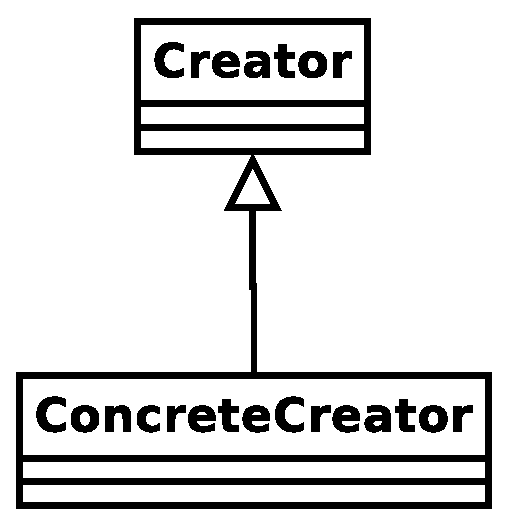
\includegraphics[width=160px]{diagrams/creational_pattern_class.eps}
					\caption{Klasės kūrimo projektavimo šablono diagrama}
					\label{fig:creational_class_pattern}
				\end{figure}

		\subsection{Abstract factory šablonas}

			Abstract factory šablonas yra projektavimo šablonas, kuris leidžia apimti skirtingus objektus su skirtingais \textit{factory} į vieną objektą. Standartiniu atveju, programuotojas įgyvendina \textit{abstract factory} ir paskui naudoja bendrą sąsają objektams kurti. Tokiu atveju programuotojui nereikia žinoti specifinių reikalavimų objektui sukurti. Objektai yra sukuriami per \textit{factory}, ir būtent \textit{factory} pasirūpina objektų reikalavimais. Šablonas atskirai objekto kūrimo specifikas nuo objekto naudojimo specifikos.

			\subsubsection{Apibrėžimas}

				Bendrinis apibrėžimas gali būti aprašytas taip -- sąsajos suteikimas, kurios pagalba galima kurti objektus, nežinant jų kūrimo specifikos.

			\subsubsection{Naudojimas}

				\textit{Factory} nusako kokie būtent yra reikalavimai objekto sukūrimui ir būtent šioje vietoje objektas yra sukuriamas. Klientui yra grąžinamas to objekto abstrakti nuoroda. Taip yra išvengiama kliento pusėje kurti iš \textit{factory} metodo gražinamo objekto kopiją. Taip pat, klientas taip visiškai nežino kokie yra sukurto objekto posistemėje esantys objektai.

				Per \textit{factory} sukuriamų objektų posistemės papildymas yra labai lengvas uždavinys. Klientas visiškai gali nežinoti ar sukuriamo objekto posistemės reikalavimai pasikeitė bet kokiu laiko momentu. Taip labai sumažėja laiko sąnaudos objekto modifikacijomis.

			\subsubsection{Struktūra}

				Šablono struktūra pateikiama \ref{fig:abstract_factory_pattern} pav. \textit{Factories} yra aprašomi visi \textit{factory methods}, kurie sukuria naujus objektus, \textit{products}.

				\begin{figure}[t]
					\centering
					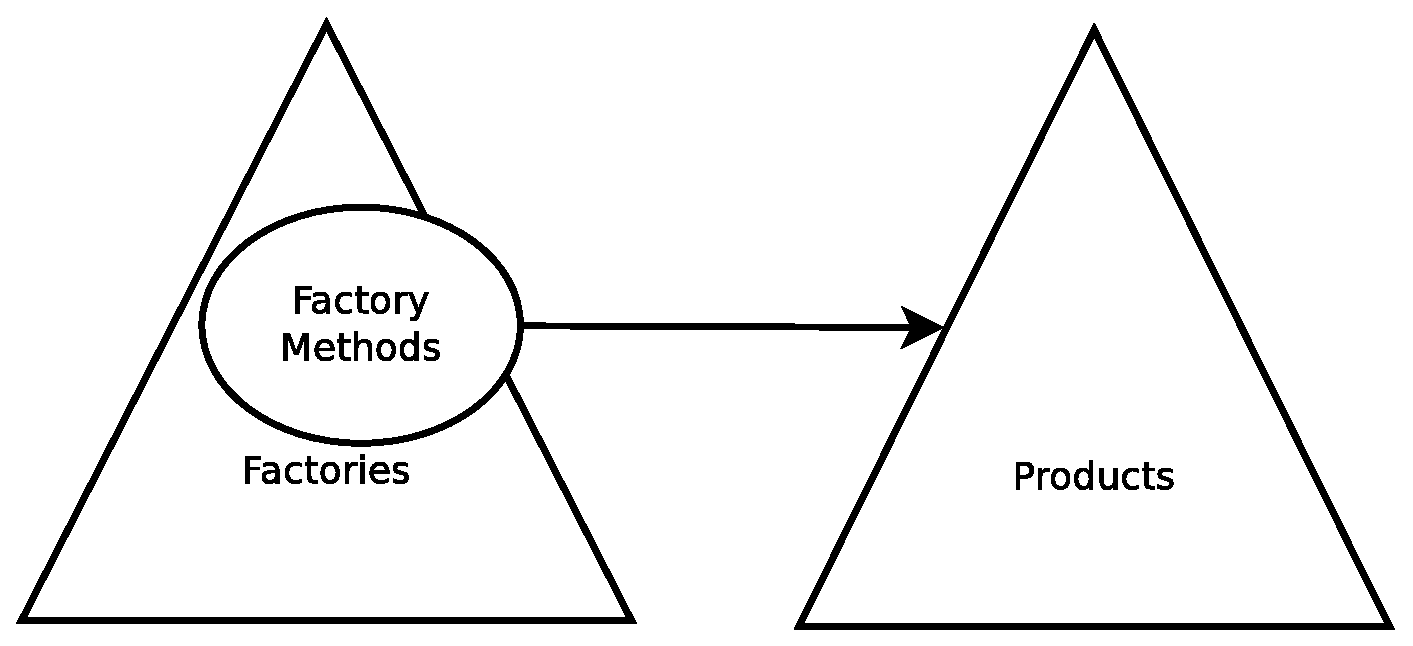
\includegraphics[width=160px]{diagrams/abstract_factory_pattern.eps}
					\caption{Abstract factory projektavimo šablono struktūra}
					\label{fig:abstract_factory_pattern}
				\end{figure}

		\subsection{Builder šablonas}

			Šablono tikslas yra objekto kūrimo reikalavimų skaldymas į žingsnius. Taip objekto kūrimas gali būti skirtingas, priklausomai nuo praeitų žingsnių, to objekto kūrimo metu.

			\subsubsection{Apibrėžimas}

				\textit{Builder} šablono tikslas yra atskirti objekto pateikimą, nuo kompleksinio objekto kūrimo. Tai įgyvendinus, kiekvienas kuriamas objektas gali būti skirtingas, priklausomai nuo kūrimo proceso.

			\subsubsection{Naudojimas}

				Šablonas yra dažnai taikomas, kuomet egzistuoja labai panašios objektų grupės, kurios skiriasi tik tam tikrų objekto parametrų būsena.

			\subsubsection{Struktūra}

				Šablono struktūra pateikiama \ref{fig:builder_pattern} pav. \textit{Builder} suteikia abstrakčią sąsaja objekto kūrimui. \textit{Concrete Builder} suteikia \textit{Builder} realizaciją. Tai yra objektas, kuris geba kurti kitus objektus. 

				\begin{figure}[t]
					\centering
					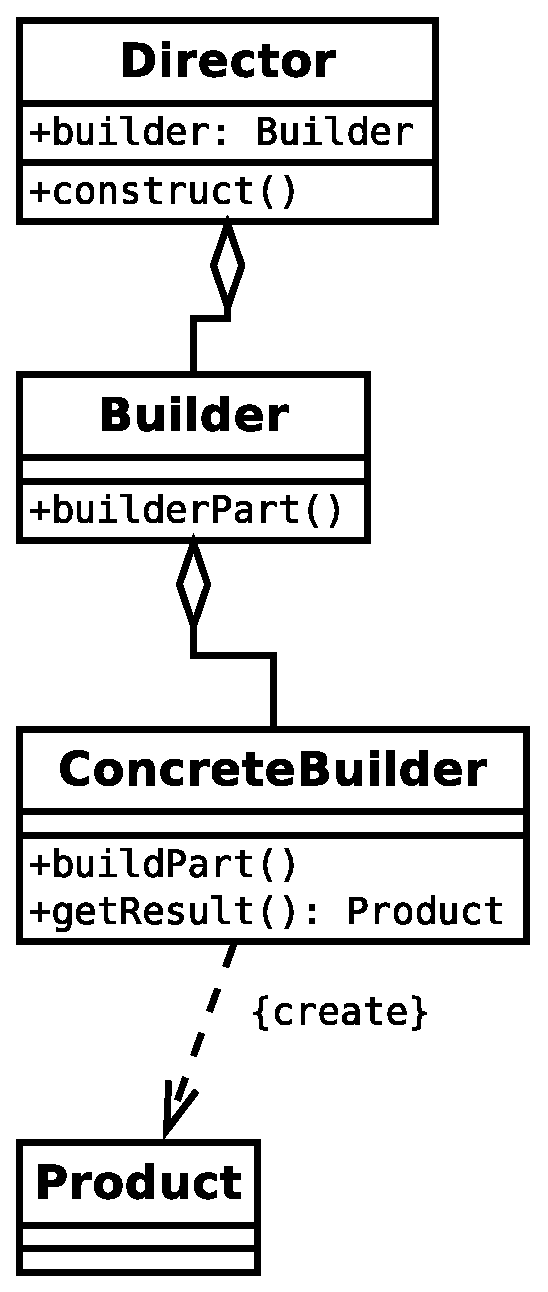
\includegraphics[width=160px]{diagrams/builder_pattern.eps}
					\caption{Builder projektavimo šablono struktūra}
					\label{fig:builder_pattern}
				\end{figure}

		\subsection{Factory method šablonas}

			\textit{Factory method} šablonas yra objektiškai orientuotas projektavimo šablonas, kuris įgyvendina fabrikų koncepciją. Objekto sukūrimas yra labai kompleksinė operacija, kurios diegimas nėra pati paprasčiausia procedūra. Taip pat, procesas gali sudaryti galimybių, labai dažnai kartoti tą patį kodą skirtingose vietose. Gali kilti tokių situacijų, kai objekto paveldimas objektas turi priklausomybių, kurios nėra pasiekiamos iš kuriamo objekto. \textit{Factory method} šablonas sprendžia tokias problemas, apibrėžiant objekto kūrimo metodą, kuris pasirūpina visomis objekto kūrimo specifikomis. 

			\subsubsection{Apibrėžimas}

				\textit{Factory method} šablonas apibrėžiamas kaip objekto kūrimo sąsajos įgyvendinimas, kuris leidžia nusakyti kokia objekto klasė yra paveldima.

			\subsubsection{Naudojimas}

				Šablonas gali būti naudojamas:
				\begin{itemize}
					\item Pakartotinio sukurto objekto panaudojimui skirtingose sistemos vietose
					\item Situacijose, kuomet objekto kūrimui reikalinga labai specifinė informacija ar informacijos šaltinis
					\item Objekto egzistavimo laiko ribojimo centralizavimui.
				\end{itemize}

			\subsubsection{Struktūra}

				Struktūra yra tokia pati, kaip ir \textit{Abstract Factory} šablono atveju. Skirtumas tik grąžinamos klasės paveldimumas.

		\subsection{Lazy initialization šablonas}

			\textit{Lazy initialization} šablonas yra metodika, kuomet specialiai yra delsiamas objekto kūrimas iki tol, kol to objekto prireikia kažkokio sistemos žingsnio metu. Metodika dažniausiai yra realizuojama saugant vėliavos kintamąjį, kuris nusako ar objektas buvo sukurtas ar ne. Kiekvieną kartą, kai yra kviečiamas objektas, tikrinamas vėliavos statusas. Jeigu vėliava sako, kad objektas jau yra sukurtas, grąžinamas objekto atvaizdas, jeigu objektas nebuvo sukurtas -- pradedamas objekto kūrimas.

			\subsubsection{Apibrėžimas}

				Objekto kūrimo specialus delsimas iki to laiko, kol objekto prireikia sistemos veikimo metu.

			\subsubsection{Naudojimas}

				\textit{Lazy initialization} dažniausiai naudojamas, kuomet reikia atlikti kažkokią sudėtingą operaciją, arba įvykdyti procesą, kuris reikalauja labai daug resursų.

			\subsubsection{Struktūra}

				Šablonas struktūros neturi.

		\subsection{Multiton šablnas}

			Šablonas yra labai panašus į \textit{Singleton} šabloną, kuris naudojamas vieno objekto atvaizdui sistemoje palaikyti. Skirtumas tarp dviejų šablonų yra toks, kad \textit{Singleton} saugo tik vieną klasės atvaizdą, o \textit{Multiton} saugo kelių klasių atvaizdą žemėlapyje.

			Šablono pagrindinis trūkumas yra sudėtingesnis testavimas, kadangi sistemoje pateikiama globali būsena. Jeigu programavimo kalboje vyrauja šiukšlių rinkimo mechanizmas, tokia metodika gali privesti prie atminties nutekėjimo.

			\subsubsection{Apibrėžimas}

				Kelių vieno atvaizdo objektų saugojimas žemėlapyje.

			\subsubsection{Naudojimas}

				Potencialus šablono naudojimas yra pateikiamas lygiagrečiai veikiančioje sistemoje, kuomet skirtingoms gijoms reikia pateikti resursų rinkinį, kurį reikia kontroliuoti.

			\subsubsection{Struktūra}

				Šablonas struktūros neturi.

		\subsection{Object pool šablonas}

			

			\subsubsection{Apibrėžimas}

			\subsubsection{Naudojimas}

			\subsubsection{Struktūra}

		\subsection{Prototype šablonas}

			\subsubsection{Apibrėžimas}

			\subsubsection{Naudojimas}

			\subsubsection{Struktūra}

		\subsection{Singleton šablonas}

			\subsubsection{Apibrėžimas}

			\subsubsection{Naudojimas}

			\subsubsection{Struktūra}

	\section{Struktūriniai šablonai}

		\subsection{Adapter šablonas}

			\subsubsection{Apibrėžimas}

			\subsubsection{Naudojimas}

			\subsubsection{Struktūra}

		\subsection{Bridge šablonas}

			\subsubsection{Apibrėžimas}

			\subsubsection{Naudojimas}

			\subsubsection{Struktūra}

		\subsection{Composite šablonas}

			\subsubsection{Apibrėžimas}

			\subsubsection{Naudojimas}

			\subsubsection{Struktūra}

		\subsection{Dekorator šablonas}

			\subsubsection{Apibrėžimas}

			\subsubsection{Naudojimas}

			\subsubsection{Struktūra}

		\subsection{Facade šablonas}

			\subsubsection{Apibrėžimas}

			\subsubsection{Naudojimas}

			\subsubsection{Struktūra}

		\subsection{Front Controller šablonas}

			\subsubsection{Apibrėžimas}

			\subsubsection{Naudojimas}

			\subsubsection{Struktūra}

		\subsection{Flyweight šablonas}

			\subsubsection{Apibrėžimas}

			\subsubsection{Naudojimas}

			\subsubsection{Struktūra}

		\subsection{Proxy šablonas}

			\subsubsection{Apibrėžimas}

			\subsubsection{Naudojimas}

			\subsubsection{Struktūra}
		
	\section{Eglesio šablonai}

		\subsection{Elgesio šablonas}

			\subsubsection{Apibrėžimas}

			\subsubsection{Naudojimas}

			\subsubsection{Struktūra}

		\subsection{Chain-of-Responsibility šablonas}

			\subsubsection{Apibrėžimas}

			\subsubsection{Naudojimas}

			\subsubsection{Struktūra}

		\subsection{Command šablonas}

			\subsubsection{Apibrėžimas}

			\subsubsection{Naudojimas}

			\subsubsection{Struktūra}

		\subsection{Interpreter šablonas}

			\subsubsection{Apibrėžimas}

			\subsubsection{Naudojimas}

			\subsubsection{Struktūra}

		\subsection{Interator šablonas}

			\subsubsection{Apibrėžimas}

			\subsubsection{Naudojimas}

			\subsubsection{Struktūra}

		\subsection{Mediator šablonas}

			\subsubsection{Apibrėžimas}

			\subsubsection{Naudojimas}

			\subsubsection{Struktūra}

		\subsection{Memento šablonas}

			\subsubsection{Apibrėžimas}

			\subsubsection{Naudojimas}

			\subsubsection{Struktūra}

		\subsection{Null Object šablonas}

			\subsubsection{Apibrėžimas}

			\subsubsection{Naudojimas}

			\subsubsection{Struktūra}

		\subsection{Observer šablonas}

			\subsubsection{Apibrėžimas}

			\subsubsection{Naudojimas}

			\subsubsection{Struktūra}

		
		\subsection{Publish/Subscribe šablonas}

			\subsubsection{Apibrėžimas}

			\subsubsection{Naudojimas}

			\subsubsection{Struktūra}

		
		\subsection{Servant šablonas}

			\subsubsection{Apibrėžimas}

			\subsubsection{Naudojimas}

			\subsubsection{Struktūra}

		\subsection{Specification šablonas}

			\subsubsection{Apibrėžimas}

			\subsubsection{Naudojimas}

			\subsubsection{Struktūra}


		\subsection{State šablonas}

			\subsubsection{Apibrėžimas}

			\subsubsection{Naudojimas}

			\subsubsection{Struktūra}


		\subsection{Strategy šablonas}

			\subsubsection{Apibrėžimas}

			\subsubsection{Naudojimas}

			\subsubsection{Struktūra}

		
		\subsection{Template method šablonas}

			\subsubsection{Apibrėžimas}

			\subsubsection{Naudojimas}

			\subsubsection{Struktūra}

		\subsection{Visitor šablonas}

			\subsubsection{Apibrėžimas}

			\subsubsection{Naudojimas}

			\subsubsection{Struktūra}

	\section{Lygiagretūs šablonai}

		\subsection{Lygiagretus šablonas}

			\subsubsection{Apibrėžimas}

			\subsubsection{Naudojimas}

			\subsubsection{Struktūra}

		\subsection{Active Object šablonas}

			\subsubsection{Apibrėžimas}

			\subsubsection{Naudojimas}

			\subsubsection{Struktūra}

		\subsection{Balking šablonas}

			\subsubsection{Apibrėžimas}

			\subsubsection{Naudojimas}

			\subsubsection{Struktūra}

		\subsection{Messaging šablonas}

			\subsubsection{Apibrėžimas}

			\subsubsection{Naudojimas}

			\subsubsection{Struktūra}

		\subsection{Double-checked šablonas}

			\subsubsection{Apibrėžimas}

			\subsubsection{Naudojimas}

			\subsubsection{Struktūra}

		\subsection{Asinchroninio metodo kreipimo šablonas}

			\subsubsection{Apibrėžimas}

			\subsubsection{Naudojimas}

			\subsubsection{Struktūra}
		
		\subsection{Saugomas sulaikymas}

			\subsubsection{Apibrėžimas}

			\subsubsection{Naudojimas}

			\subsubsection{Struktūra}

		\subsection{Uždarymas}

			\subsubsection{Apibrėžimas}

			\subsubsection{Naudojimas}

			\subsubsection{Struktūra}

		\subsection{Stebėjimas}

			\subsubsection{Apibrėžimas}

			\subsubsection{Naudojimas}

			\subsubsection{Struktūra}

		\subsection{Reactor šablonas}

			\subsubsection{Apibrėžimas}

			\subsubsection{Naudojimas}

			\subsubsection{Struktūra}

		\subsection{Scheduler šablonas}

			\subsubsection{Apibrėžimas}

			\subsubsection{Naudojimas}

			\subsubsection{Struktūra}

		\subsection{Thread pool šablonas}

			\subsubsection{Apibrėžimas}

			\subsubsection{Naudojimas}

			\subsubsection{Struktūra}

\end{document}